\documentclass[journal,12pt,twocolumn]{IEEEtran}
%
\usepackage{setspace}
\usepackage{gensymb}
%\doublespacing
\singlespacing

%\usepackage{graphicx}
%\usepackage{amssymb}
%\usepackage{relsize}
\usepackage[cmex10]{amsmath}
%\usepackage{amsthm}
%\interdisplaylinepenalty=2500
%\savesymbol{iint}
%\usepackage{txfonts}
%\restoresymbol{TXF}{iint}
%\usepackage{wasysym}
\usepackage{amsthm}
%\usepackage{iithtlc}
\usepackage{mathrsfs}
\usepackage{txfonts}
\usepackage{stfloats}
\usepackage{bm}
\usepackage{cite}
\usepackage{cases}
\usepackage{subfig}
%\usepackage{xtab}
\usepackage{longtable}
\usepackage{multirow}
%\usepackage{algorithm}
%\usepackage{algpseudocode}
\usepackage{enumitem}
\usepackage{mathtools}
\usepackage{steinmetz}
\usepackage{tikz}
\usepackage[american]{circuitikz}
\usepackage{verbatim}
\usepackage{tfrupee}
\usepackage[breaklinks=true]{hyperref}
%\usepackage{stmaryrd}
\usepackage{tkz-euclide} % loads  TikZ and tkz-base
\usetkzobj{all}
\usetikzlibrary{decorations.markings}
\usetikzlibrary{shapes.geometric}
\newif\iflabrev
\usepackage{listings}
    \usepackage{color}                                            %%
    \usepackage{array}                                            %%
    \usepackage{longtable}                                        %%
    \usepackage{calc}                                             %%
    \usepackage{multirow}                                         %%
    \usepackage{hhline}                                           %%
    \usepackage{ifthen}                                           %%
  %optionally (for landscape tables embedded in another document): %%
    \usepackage{lscape}     
\usepackage{multicol}
\usepackage{chngcntr}
%\usepackage{enumerate}

%\usepackage{wasysym}
%\newcounter{MYtempeqncnt}
\DeclareMathOperator*{\Res}{Res}
%\renewcommand{\baselinestretch}{2}
\renewcommand\thesection{\arabic{section}}
\renewcommand\thesubsection{\thesection.\arabic{subsection}}
\renewcommand\thesubsubsection{\thesubsection.\arabic{subsubsection}}

\renewcommand\thesectiondis{\arabic{section}}
\renewcommand\thesubsectiondis{\thesectiondis.\arabic{subsection}}
\renewcommand\thesubsubsectiondis{\thesubsectiondis.\arabic{subsubsection}}

% correct bad hyphenation here
\hyphenation{op-tical net-works semi-conduc-tor}
\def\inputGnumericTable{}                                 %%

\lstset{
%language=C,
frame=single, 
breaklines=true,
columns=fullflexible
}
%\lstset{
%language=tex,
%frame=single, 
%breaklines=true
%}

\begin{document}
%


\newtheorem{theorem}{Theorem}[section]
\newtheorem{problem}{Problem}
\newtheorem{proposition}{Proposition}[section]
\newtheorem{lemma}{Lemma}[section]
\newtheorem{corollary}[theorem]{Corollary}
\newtheorem{example}{Example}[section]
\newtheorem{definition}[problem]{Definition}
%\newtheorem{thm}{Theorem}[section] 
%\newtheorem{defn}[thm]{Definition}
%\newtheorem{algorithm}{Algorithm}[section]
%\newtheorem{cor}{Corollary}
\newcommand{\BEQA}{\begin{eqnarray}}
\newcommand{\EEQA}{\end{eqnarray}}
\newcommand{\define}{\stackrel{\triangle}{=}}
\bibliographystyle{IEEEtran}
%\bibliographystyle{ieeetr}
\providecommand{\mbf}{\mathbf}
\providecommand{\pr}[1]{\ensuremath{\Pr\left(#1\right)}}
\providecommand{\qfunc}[1]{\ensuremath{Q\left(#1\right)}}
\providecommand{\sbrak}[1]{\ensuremath{{}\left[#1\right]}}
\providecommand{\lsbrak}[1]{\ensuremath{{}\left[#1\right.}}
\providecommand{\rsbrak}[1]{\ensuremath{{}\left.#1\right]}}
\providecommand{\brak}[1]{\ensuremath{\left(#1\right)}}
\providecommand{\lbrak}[1]{\ensuremath{\left(#1\right.}}
\providecommand{\rbrak}[1]{\ensuremath{\left.#1\right)}}
\providecommand{\cbrak}[1]{\ensuremath{\left\{#1\right\}}}
\providecommand{\lcbrak}[1]{\ensuremath{\left\{#1\right.}}
\providecommand{\rcbrak}[1]{\ensuremath{\left.#1\right\}}}
\theoremstyle{remark}
\newtheorem{rem}{Remark}
\newcommand{\sgn}{\mathop{\mathrm{sgn}}}
\providecommand{\abs}[1]{\left\vert#1\right\vert}
\providecommand{\res}[1]{\Res\displaylimits_{#1}} 
\providecommand{\norm}[1]{\left\lVert#1\right\rVert}
%\providecommand{\norm}[1]{\lVert#1\rVert}
\providecommand{\mtx}[1]{\mathbf{#1}}
\providecommand{\mean}[1]{E\left[ #1 \right]}
\providecommand{\fourier}{\overset{\mathcal{F}}{ \rightleftharpoons}}
%\providecommand{\hilbert}{\overset{\mathcal{H}}{ \rightleftharpoons}}
\providecommand{\system}{\overset{\mathcal{H}}{ \longleftrightarrow}}
	%\newcommand{\solution}[2]{\textbf{Solution:}{#1}}
\newcommand{\solution}{\noindent \textbf{Solution: }}
\newcommand{\cosec}{\,\text{cosec}\,}
\providecommand{\dec}[2]{\ensuremath{\overset{#1}{\underset{#2}{\gtrless}}}}
\newcommand{\myvec}[1]{\ensuremath{\begin{pmatrix}#1\end{pmatrix}}}
\newcommand{\mydet}[1]{\ensuremath{\begin{vmatrix}#1\end{vmatrix}}}
%\numberwithin{equation}{section}
\numberwithin{equation}{subsection}
%\numberwithin{problem}{section}
%\numberwithin{definition}{section}
\makeatletter
\@addtoreset{figure}{problem}
\makeatother
\let\StandardTheFigure\thefigure
\let\vec\mathbf
%\renewcommand{\thefigure}{\theproblem.\arabic{figure}}
\renewcommand{\thefigure}{\theproblem}
%\setlist[enumerate,1]{before=\renewcommand\theequation{\theenumi.\arabic{equation}}
%\counterwithin{equation}{enumi}
%\renewcommand{\theequation}{\arabic{subsection}.\arabic{equation}}
\def\putbox#1#2#3{\makebox[0in][l]{\makebox[#1][l]{}\raisebox{\baselineskip}[0in][0in]{\raisebox{#2}[0in][0in]{#3}}}}
     \def\rightbox#1{\makebox[0in][r]{#1}}
     \def\centbox#1{\makebox[0in]{#1}}
     \def\topbox#1{\raisebox{-\baselineskip}[0in][0in]{#1}}
     \def\midbox#1{\raisebox{-0.5\baselineskip}[0in][0in]{#1}}
\vspace{3cm}
\title{
%	\logo{
Closed loop gain and Phase Margin
%	}
}
\author{ Ganraj Borade$^{*}$\\ { ee18btech11016@iith.ac.in}% <-this % stops a space
	\thanks{*The author is with the Department
		of Electrical Engineering, Indian Institute of Technology, Hyderabad
		502285 India. All content in this manual is released under GNU GPL.  Free and open source.}
	
}	
%\title{
%	\logo{Matrix Analysis through Octave}{\begin{center}\includegraphics[scale=.24]{tlc}\end{center}}{}{HAMDSP}
%}
% paper title
% can use linebreaks \\ within to get better formatting as desired
%\title{Matrix Analysis through Octave}
%
%
% author names and IEEE memberships
% note positions of commas and nonbreaking spaces ( ~ ) LaTeX will not break
% a structure at a ~ so this keeps an author's name from being broken across
% two lines.
% use \thanks{} to gain access to the first footnote area
% a separate \thanks must be used for each paragraph as LaTeX2e's \thanks
% was not built to handle multiple paragraphs
%
%\author{<-this % stops a space
%\thanks{}}
%}
% note the % following the last \IEEEmembership and also \thanks - 
% these prevent an unwanted space from occurring between the last author name
% and the end of the author line. i.e., if you had this:
% 
% \author{....lastname \thanks{...} \thanks{...} }
%                     ^------------^------------^----Do not want these spaces!
%
% a space would be appended to the last name and could cause every name on that
% line to be shifted left slightly. This is one of those "LaTeX things". For
% instance, "\textbf{A} \textbf{B}" will typeset as "A B" not "AB". To get
% "AB" then you have to do: "\textbf{A}\textbf{B}"
% \thanks is no different in this regard, so shield the last } of each \thanks
% that ends a line with a % and do not let a space in before the next \thanks.
% Spaces after \IEEEmembership other than the last one are OK (and needed) as
% you are supposed to have spaces between the names. For what it is worth,
% this is a minor point as most people would not even notice if the said evil
% space somehow managed to creep in.
% The paper headers
%\markboth{Journal of \LaTeX\ Class Files,~Vol.~6, No.~1, January~2007}%
%{Shell \MakeLowercase{\textit{et al.}}: Bare Demo of IEEEtran.cls for Journals}
% The only time the second header will appear is for the odd numbered pages
% after the title page when using the twoside option.
% 
% *** Note that you probably will NOT want to include the author's ***
% *** name in the headers of peer review papers.                   ***
% You can use \ifCLASSOPTIONpeerreview for conditional compilation here if
% you desire.
% If you want to put a publisher's ID mark on the page you can do it like
% this:
%\IEEEpubid{0000--0000/00\$00.00~\copyright~2007 IEEE}
% Remember, if you use this you must call \IEEEpubidadjcol in the second
% column for its text to clear the IEEEpubid mark.
% make the title area
\maketitle
\newpage
%\tableofcontents
\bigskip
\renewcommand{\thefigure}{\theenumi}
\renewcommand{\thetable}{\theenumi}
%\renewcommand{\theequation}{\theenumi}
%\begin{abstract}
%%\boldmath
%In this letter, an algorithm for evaluating the exact analytical bit error rate  (BER)  for the piecewise linear (PL) combiner for  multiple relays is presented. Previous results were available only for upto three relays. The algorithm is unique in the sense that  the actual mathematical expressions, that are prohibitively large, need not be explicitly obtained. The diversity gain due to multiple relays is shown through plots of the analytical BER, well supported by simulations. 
%
%\end{abstract}
% IEEEtran.cls defaults to using nonbold math in the Abstract.
% This preserves the distinction between vectors and scalars. However,
% if the journal you are submitting to favors bold math in the abstract,
% then you can use LaTeX's standard command \boldmath at the very start
% of the abstract to achieve this. Many IEEE journals frown on math
% in the abstract anyway.
% Note that keywords are not normally used for peerreview papers.
%\begin{IEEEkeywords}
%Cooperative diversity, decode and forward, piecewise linear
%\end{IEEEkeywords}
% For peer review papers, you can put extra information on the cover
% page as needed:
% \ifCLASSOPTIONpeerreview
% \begin{center} \bfseries EDICS Category: 3-BBND \end{center}
% \fi
%
% For peerreview papers, this IEEEtran command inserts a page break and
% creates the second title. It will be ignored for other modes.
%\IEEEpeerreviewmaketitle
%\begin{abstract}
%This manual is an introduction to control systems in feedback circuits. Links to sample Python codes are available in the text.  
%\end{abstract}
%Download python codes using 
%\begin{lstlisting}
%svn co https://github.com/gadepall/school/trunk/control/feedback/codes
%\end{lstlisting}
%\section{Feedback Voltage Amplifier: Series-Shunt}
%\input{./chapters/ee18btech11005.tex}
%
%\section{Feedback Current Amplifier: Shunt-Series}
%\input{./chapters/ee18btech11021.tex}
%
%\section{Feedback Current Amplifier: Shunt-Series}
%\subsection{Ideal Case}
%\input{./chapters/ee18btech11014.tex}
%\subsection{Practical Case}
An amplifier has a dc gain of $10^5$ and poles at $10^5$ Hz , $3.16 \times 10^5$ Hz and $10^6$ Hz . Find the value of $\beta$,and the corresponding closed-loop gain , for which a phase margin of $45\degree$ is obtained. 

\begin{enumerate}[label=\arabic*.,ref=\theenumi]
\numberwithin{equation}{enumi}

\item Find the transfer function of the three pole OPAMP.
\\
\solution 
For a 3-pole amplifier open loop transfer function is 
\begin{align}
G(s) = \frac{G_0}{\brak{1+\frac{s}{P_{1}}}\brak{1+\frac{s}{P_{2}}}\brak{1+\frac{s}{P_{3}}}}
\end{align}

where the Gain and Poles are listed in Table \ref{table:ee18btech11016_Table_1}.
%
\begin{table}[!ht]
\centering


%%  This section checks if we are begin input into another file or  %%
%%  the file will be compiled alone. First use a macro taken from   %%
%%  the TeXbook ex 7.7 (suggestion of Han-Wen Nienhuys).            %%
\def\ifundefined#1{\expandafter\ifx\csname#1\endcsname\relax}


%%  Check for the \def token for inputed files. If it is not        %%
%%  defined, the file will be processed as a standalone and the     %%
%%  preamble will be used.                                          %%
\ifundefined{inputGnumericTable}

%%  We must be able to close or not the document at the end.        %%
	\def\gnumericTableEnd{\end{document}}


%%%%%%%%%%%%%%%%%%%%%%%%%%%%%%%%%%%%%%%%%%%%%%%%%%%%%%%%%%%%%%%%%%%%%%
%%                                                                  %%
%%  This is the PREAMBLE. Change these values to get the right      %%
%%  paper size and other niceties.                                  %%
%%                                                                  %%
%%%%%%%%%%%%%%%%%%%%%%%%%%%%%%%%%%%%%%%%%%%%%%%%%%%%%%%%%%%%%%%%%%%%%%

	\documentclass[12pt%
			  %,landscape%
                    ]{report}
       \usepackage[latin1]{inputenc}
       \usepackage{fullpage}
       \usepackage{color}
       \usepackage{array}
       \usepackage{longtable}
       \usepackage{calc}
       \usepackage{multirow}
       \usepackage{hhline}
       \usepackage{ifthen}
%%  End of the preamble for the standalone. The next section is for %%
%%  documents which are included into other LaTeX2e files.          %%
\else

%%  We are not a stand alone document. For a regular table, we will %%
%%  have no preamble and only define the closing to mean nothing.   %%
    \def\gnumericTableEnd{}

%%  If we want landscape mode in an embedded document, comment out  %%
%%  the line above and uncomment the two below. The table will      %%
%%  begin on a new page and run in landscape mode.                  %%
%       \def\gnumericTableEnd{\end{landscape}}
%       \begin{landscape}


%%  End of the else clause for this file being \input.              %%
\fi

%%%%%%%%%%%%%%%%%%%%%%%%%%%%%%%%%%%%%%%%%%%%%%%%%%%%%%%%%%%%%%%%%%%%%%
%%                                                                  %%
%%  The rest is the gnumeric table, except for the closing          %%
%%  statement. Changes below will alter the table's appearance.     %%
%%                                                                  %%
%%%%%%%%%%%%%%%%%%%%%%%%%%%%%%%%%%%%%%%%%%%%%%%%%%%%%%%%%%%%%%%%%%%%%%

\providecommand{\gnumericmathit}[1]{#1} 
%%  Uncomment the next line if you would like your numbers to be in %%
%%  italics if they are italizised in the gnumeric table.           %%
%\renewcommand{\gnumericmathit}[1]{\mathit{#1}}
\providecommand{\gnumericPB}[1]%
{\let\gnumericTemp=\\#1\let\\=\gnumericTemp\hspace{0pt}}
 \ifundefined{gnumericTableWidthDefined}
        \newlength{\gnumericTableWidth}
        \newlength{\gnumericTableWidthComplete}
        \newlength{\gnumericMultiRowLength}
        \global\def\gnumericTableWidthDefined{}
 \fi
%% The following setting protects this code from babel shorthands.  %%
 \ifthenelse{\isundefined{\languageshorthands}}{}{\languageshorthands{english}}
%%  The default table format retains the relative column widths of  %%
%%  gnumeric. They can easily be changed to c, r or l. In that case %%
%%  you may want to comment out the next line and uncomment the one %%
%%  thereafter                                                      %%
\providecommand\gnumbox{\makebox[0pt]}
%%\providecommand\gnumbox[1][]{\makebox}

%% to adjust positions in multirow situations                       %%
\setlength{\bigstrutjot}{\jot}
\setlength{\extrarowheight}{\doublerulesep}

%%  The \setlongtables command keeps column widths the same across  %%
%%  pages. Simply comment out next line for varying column widths.  %%
\setlongtables

\setlength\gnumericTableWidth{%
	60pt+%
	100pt+%
0pt}
\def\gumericNumCols{2}
\setlength\gnumericTableWidthComplete{\gnumericTableWidth+%
         \tabcolsep*\gumericNumCols*2+\arrayrulewidth*\gumericNumCols}
\ifthenelse{\lengthtest{\gnumericTableWidthComplete > \linewidth}}%
         {\def\gnumericScale{\ratio{\linewidth-%
                        \tabcolsep*\gumericNumCols*2-%
                        \arrayrulewidth*\gumericNumCols}%
{\gnumericTableWidth}}}%
{\def\gnumericScale{1}}

%%%%%%%%%%%%%%%%%%%%%%%%%%%%%%%%%%%%%%%%%%%%%%%%%%%%%%%%%%%%%%%%%%%%%%
%%                                                                  %%
%% The following are the widths of the various columns. We are      %%
%% defining them here because then they are easier to change.       %%
%% Depending on the cell formats we may use them more than once.    %%
%%                                                                  %%
%%%%%%%%%%%%%%%%%%%%%%%%%%%%%%%%%%%%%%%%%%%%%%%%%%%%%%%%%%%%%%%%%%%%%%

\ifthenelse{\isundefined{\gnumericColA}}{\newlength{\gnumericColA}}{}\settowidth{\gnumericColA}{\begin{tabular}{@{}p{60pt*\gnumericScale}@{}}x\end{tabular}}
\ifthenelse{\isundefined{\gnumericColB}}{\newlength{\gnumericColB}}{}\settowidth{\gnumericColB}{\begin{tabular}{@{}p{100pt*\gnumericScale}@{}}x\end{tabular}}
\begin{tabular}[c]{%
	b{\gnumericColA}%
	b{\gnumericColB}%%
	}

%%%%%%%%%%%%%%%%%%%%%%%%%%%%%%%%%%%%%%%%%%%%%%%%%%%%%%%%%%%%%%%%%%%%%%
%%  The longtable options. (Caption, headers... see Goosens, p.124) %%
%	\caption{The Table Caption.}             \\	%
% \hline	% Across the top of the table.
%%  The rest of these options are table rows which are placed on    %%
%%  the first, last or every page. Use \multicolumn if you want.    %%

%%  Header for the first page.                                      %%
%	\multicolumn{3}{c}{The First Header} \\ \hline 
%	\multicolumn{1}{c}{colTag}	%Column 1
%	&\multicolumn{1}{c}{colTag}	%Column 2
%	&\multicolumn{1}{c}{colTag}	\\ \hline %Last column
%	\endfirsthead

%%  The running header definition.                                  %%
%	\hline
%	\multicolumn{3}{l}{\ldots\small\slshape continued} \\ \hline
%	\multicolumn{1}{c}{colTag}	%Column 1
%	&\multicolumn{1}{c}{colTag}	%Column 2
%	&\multicolumn{1}{c}{colTag}	\\ \hline %Last column
%	\endhead

%%  The running footer definition.                                  %%
%	\hline
%	\multicolumn{3}{r}{\small\slshape continued\ldots} \\
%	\endfoot

%%  The ending footer definition.                                   %%
%	\multicolumn{3}{c}{That's all folks} \\ \hline 
%	\endlastfoot
%%%%%%%%%%%%%%%%%%%%%%%%%%%%%%%%%%%%%%%%%%%%%%%%%%%%%%%%%%%%%%%%%%%%%%

\hhline{|-|-}
	 \multicolumn{1}{|p{\gnumericColA}|}%
	{\gnumericPB{\centering}\textbf{Parameters}}
	&\multicolumn{1}{p{\gnumericColB}|}%
	{\gnumericPB{\centering}\textbf{Value}}

	
\\


\hhline{|--|}
	 \multicolumn{1}{|p{\gnumericColA}|}%
	{\gnumericPB{\centering}$P_{1}$}
	&\multicolumn{1}{p{\gnumericColB}|}%
	{\gnumericPB{\centering}$2\pi\times10^{5}$ rad/sec}


\\


\hhline{|--|}
	 \multicolumn{1}{|p{\gnumericColA}|}%
	{\gnumericPB{\centering}$P_{2}$}
	&\multicolumn{1}{p{\gnumericColB}|}%
	{\gnumericPB{\centering}$2\pi(3.16\times10^{5})$ rad/sec}


\\

\hhline{|--|}
	 \multicolumn{1}{|p{\gnumericColA}|}%
	{\gnumericPB{\centering}$P_{3}$}
	&\multicolumn{1}{p{\gnumericColB}|}%
	{\gnumericPB{\centering}$2\pi\times10^{6}$ rad/sec}


\\



\hhline{|--|}
	 \multicolumn{1}{|p{\gnumericColA}|}%
	{\gnumericPB{\centering}$G_0$}
	&\multicolumn{1}{p{\gnumericColB}|}%
	{\gnumericPB{\centering}$10^{5}$}



\\
\hhline{|-|-|}
\end{tabular}

\ifthenelse{\isundefined{\languageshorthands}}{}{\languageshorthands{\languagename}}
\gnumericTableEnd


\caption{}
\label{table:ee18btech11016_Table_1}
\end{table}

Poles are at $f_{1} =10^5$ and $f_{2} = 3.16\times10^{5}$ and $f_{3} = 10^6$ 
\begin{multline}
G\brak{f} = \frac{G_{0}}{\brak{1+\j\frac{f}{f_{1}}}\brak{1+\j\frac{f}{f_{2}}}\brak{1+\j\frac{f}{f_{3}}}}\\
= \frac{10^{5}}{\brak{1+\j\frac{f}{10^5}}\brak{1+\j\frac{f}{3.16\times10^{5}}}\brak{1+\j\frac{f}{10^6}}}
\label{eq:ee18btech11016_1}
\end{multline}
\item Find the loop gain expression ($G(s)H$) (H is constant in this question).
\\
\solution 
\begin{align}
GH = \frac{10^{5}}{\brak{1+\j\frac{f}{10^5}}\brak{1+\j\frac{f}{3.16\times10^{5}}}\brak{1+\j\frac{f}{10^6}}} . H
\label{eq:ee18btech11016_2}
\end{align}

\item Find the PM and the crossover frequency.
\\
\solution  
The phase margin = $180\degree$ - $\phi(f_{c})$ where $f_{c}$ is the frequency where $\abs{G(f)H}=1$.It is required that the phase margin is $45\degree$ , so that :

\begin{align}
45\degree &=  180\degree - \phi(f_{c}) \implies \phi(f_{c})=-135\degree.
\end{align}
From \eqref{eq:ee18btech11016_2} 
\begin{align}
-135\degree = -\tan^{-1}\brak{\frac{f_{c}}{10^5}}-\tan^{-1}\brak{\frac{f_{c}}{3.16\times10^5}}-\tan^{-1}\brak{\frac{f_{c}}{10^6}}
\end{align}
After solving the above equation , we get $f_{c}$ = 315KHz.
\\

\item Verify your result using a Bode plot.
\\
\solution  The following code  id used to verify the value of $f_{c}$ Fig. \ref{fig:ee18btech11016_1}

\begin{lstlisting}
codes/ee18btech11016/ee18btech11016_1.py
\end{lstlisting}
%
\begin{figure}[!h]
\centering
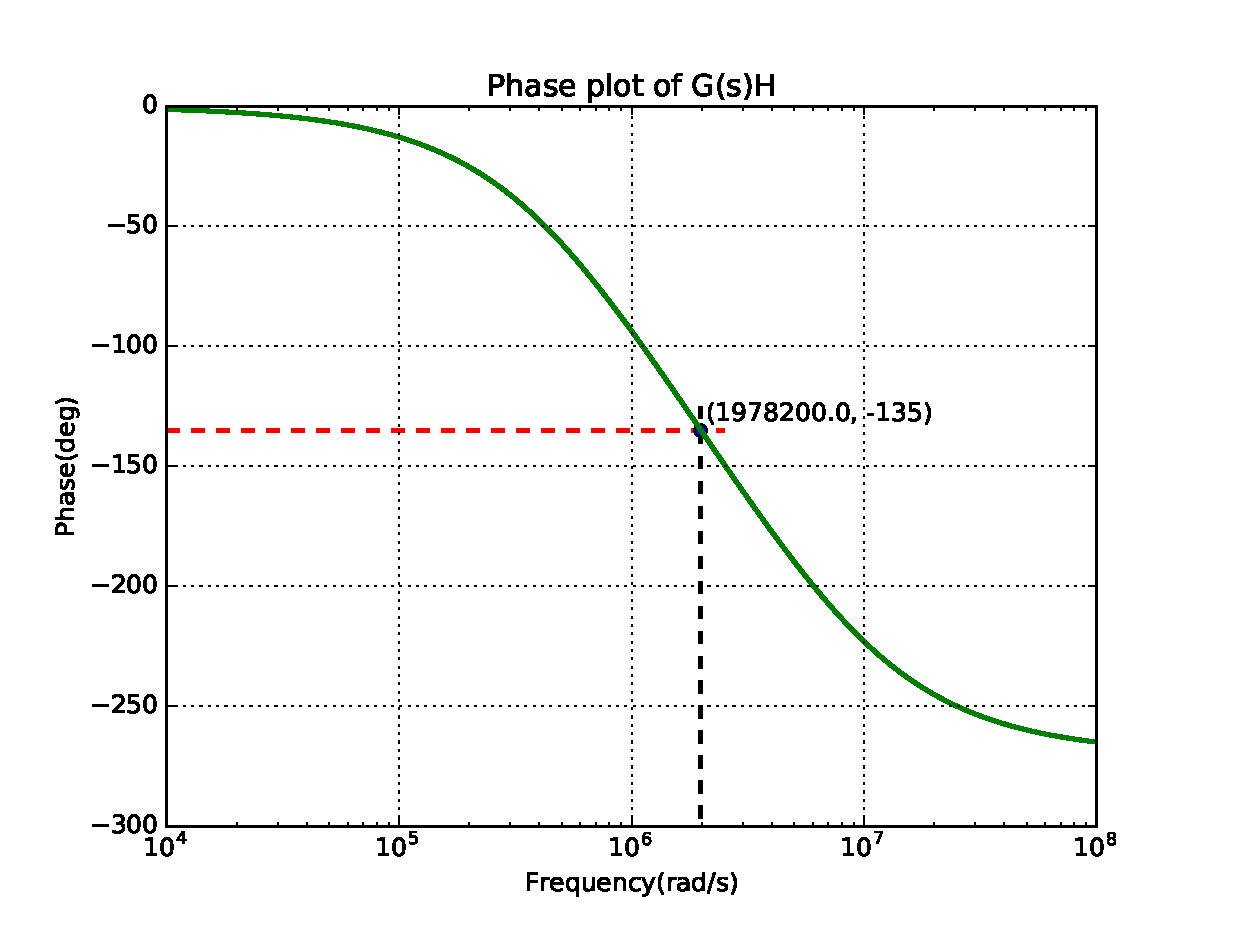
\includegraphics[width=\columnwidth]{./figs/ee18btech11016/ee18btech11016_resultbode.eps}
\caption{}
\label{fig:ee18btech11016_1}
\end{figure}

\item Find the value of H.\\
\solution From \eqref{eq:ee18btech11016_2},The magnitude of the loop gain at this frequency $f_{c}$ is given by $\abs{G(f_{c})H}$ :
 
\begin{align}
    H\brak{\frac{10^5}{\sqrt{1+(\frac{315\times10^3}{10^5})^2}\sqrt{1+(\frac{315\times10^3}{3.16\times10^6})^2}\sqrt{1+(\frac{315\times10^3}{10^6})^2}}}
\end{align}

which is equal to $H\times(20.04\times10^3)$.
So,
\begin{align}
\abs{G(f_{c})H} = H\times(20.04\times10^3)
\end{align}
Setting $\abs{G(f_{c})H}$ = 1 , Solving for $\beta$ (here $\beta$ is equal to H) yields 
\begin{align}
\beta &= 48.9\times10^{-6}
\end{align}
Or
\begin{align}
H &= 48.9\times10^{-6}
\end{align}

\item Find the corresponding closed-loop gain for which a phase margin of $45\degree$ is obtained.\\
\solution The closed loop dc gain is given as
\begin{align}
A_{f} = \frac{G_{0}}{1+HG_{0}}=\frac{10^5}{1+48.9\times10^{-6}(10^5)}
\end{align} 
\begin{align}
A_{f} = 17\times10^3
\end{align}


\item Realise the above system with $PM = 45 \degree$ using a feedback circuit.\\
\solution
\begin{figure}[ht!]
	\begin{center}
		\resizebox{\columnwidth/1}{!}{\tikzstyle{block} = [draw, rectangle, 
    minimum height=1.25em, minimum width=2.5em]
\tikzstyle{sum} = [draw, circle, node distance=1cm]
\tikzstyle{input} = [coordinate]
\tikzstyle{output} = [coordinate]
\tikzstyle{pinstyle} = [pin edge={to-,thin,black}]

% The block diagram code is probably more verbose than necessary
\begin{tikzpicture}[auto, node distance=2.5cm,>=latex']
    % We start by placing the blocks
    \node [input, name=input] {};
    \node [sum, right of=input] (sum) {};
    \node [block, right of=sum] (controller) {$G(s)$};
    
    % We draw an edge between the controller and system block to 
    % calculate the coordinate u. We need it to place the measurement block. 
   
    \node [output, right of=controller] (output) {};
    \node [block, below of=controller] (measurements) {$48.9\times10^{-6}$};

    % Once the nodes are placed, connecting them is easy. 
    \draw [draw,->] (input) -- node[pos=0.99] {$+$} node {$V_{s}$} (sum);
    \draw [->] (sum) -- node {$V_{i}$} (controller);
    \draw [->] (controller) -- node [name=y] {$V_{o}$}(output);
    \draw [->] (y) |- (measurements);
    \draw [->] (measurements) -| node[pos=0.99] {$-$} node [near end] {$V_{f}$} (sum);
\end{tikzpicture}}
	\end{center}
	\caption{}
	\label{fig:ee18btech11016_figa}
\end{figure}

The transfer function of OPAMP is
\begin{align}
    G(s) = \frac{10^{5}}{\brak{1+\frac{s}{2\pi \times 10^5}}\brak{1+\frac{s}{2\pi \times3.16 \times 10^{5}}}\brak{1+\frac{s}{2\pi \times 10^{6}}}}
\end{align}
%
\item For the feedback gain H\\
\solution\\
Choose a resistance network such that
\begin{align}
    H = \frac{V_{f}}{V_{o}} = \frac{R_{f_{1}}}{R_{f_{1}}+R_{f_{2}}} \approx 48.9\times10^{-6}
\end{align}
\begin{figure}[ht!]
	\begin{center}
		\resizebox{\columnwidth/2}{!}{\begin{circuitikz}[american]
\ctikzset{tripoles/mos style/arrows}
\draw (1,2) to[short, -o] (0,2) node[label={below:$v_{o}$}]{};
\draw (1,2) to[R=$R_{f_{2}}$] (2,2) -- (3,2) to[R=$R_{f_{1}}$] (3,0) node[ground](GND){};
\draw (3,2) to[short, -o] (4,2) node[label={below:$v_{f}$}]{};
\end{circuitikz}}
	\end{center}
	\caption{}
	\label{fig:ee18btech11016_figb}
\end{figure}

Choose $R_{f_{1}}$ and $R_{f_{2}}$ as
\begin{align}
    R_{f_{1}} = 100\ohm\\
    R_{f_{2}} = 2.045M\ohm
\end{align}
\begin{align}
H = \frac{R_{f_{1}}}{R_{f_{1}}+R_{f_{2}}} = \frac{100}{100+2.045\times10^6} \approx 48.9\times10^{-6}
\end{align}
\item Feedback Circuit for $PM = 45\degree$
\\
\solution
\begin{figure}[ht!]
	\begin{center}
		\resizebox{\columnwidth}{!}{\begin{circuitikz}[american]

\draw (2,2)  node[op amp] (OA) {};
\draw (OA.+) -- (0,1.5) to[vsourcesin, l= $V_{s}$] (0,0) node[ground](GND){};
\draw (OA.-) -- (0,2.5) node[label={below:$V_{f}$}]{} to[R,l_=$100\ohm$] (-2,2.5) node[ground](GND){};
\draw (OA.out) -- (3,2) node[label={}]{};
\draw (3,2) -- (4.5,2) node[label={above:$V_{o}$}]{};
%\draw (3,2) to[R=$5300\ohm$] (5.5,2) node[label={}]{} to[C,l_=$3nF$] (5.5,0) node[ground](GND){};
%\draw (5.5,2) -- (6.5,2) node[label={above:$V_{o}$}]{};
\draw (3,2) -- (3,4.5) to[R=$4.057M\ohm$] (0,4.5) -- (0,2.5);
\end{circuitikz}
}
	\end{center}
	\caption{}
	\label{fig:ee18btech11016_figc}
\end{figure}

\item Simulate the circuit in ngspice.\\
\solution The following code provides instructions about the simulation.
\begin{lstlisting}
codes/ee18btech11016/spice/README.md
\end{lstlisting}


The following netlist simulates the unity feedback system. 
\\

\begin{lstlisting}
codes/ee18btech11016/spice/ee18btech1016_sim.net
\end{lstlisting}
 The step response in spice is plotted using the following code in Fig. \ref{fig:ee18btech11016_spice}
 \begin{lstlisting}
codes/ee18btech11016/spice/ee18btech11016_simulation.py
\end{lstlisting}
\begin{figure}[!h]
\centering
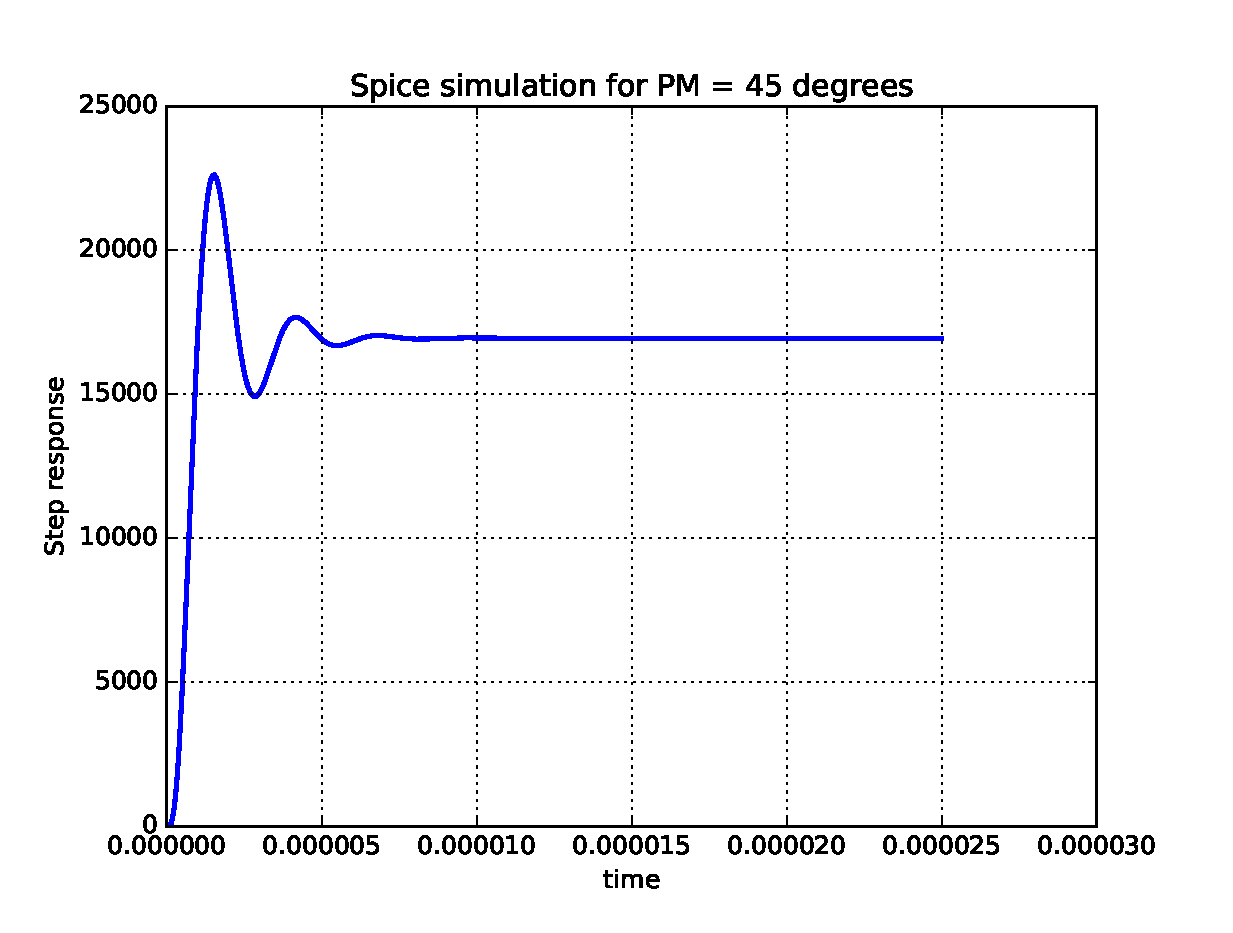
\includegraphics[width=\columnwidth]{./figs/ee18btech11016/ee18btech11016_spice.eps}
\caption{}
\label{fig:ee18btech11016_spice}
\end{figure}

\item Overview of implementation.\\
\solution Fig. \ref{fig:ee18btech110016_circuit_1} shows how the circuit is actually implemented in spice using the parameters in Table \ref{table:ee18btech11016_Table_2}  

\begin{figure}[!ht]
	\begin{center}
				\resizebox{\columnwidth}{!}{
\begin{circuitikz}
\ctikzset{bipoles/length=1cm}

\draw 
(-2,1)--(-1,1)--(-1,0) to [R = $RIN$] (-1,0)--(-1,-1)--(-2,-1)


(0, 0) to[I=$ $] (0,0) to (0,-1) %node[ground]{}
(0,0) -- (0,1)--(0.25,1) to[] (1,1) 
to [R = $R_{1}$] (1,-1) 
(1,1)--(2,1)to [C = $C1$](2,-1)
(3,-1)--(3,-1.5)node[ground]{}

(4,0)to [I=$ $] (4,0) to (4,-1)
(4,0) -- (4,1)--(4.25,1) to[] (5,1)
to [R = $R_{2}$] (5,-1) 
(5,1)--(6,1)to [C = $C2$](6,-1)


(8, 0) to[I=$ $] (8,0) to (8,-1) %node[ground]{}
(8,0) -- (8,1)--(8.25,1) to[] (9,1) 
to [R = $R_{3}$] (9,-1) 
(9,1)--(10,1)to [C = $C3$](10,-1)
(0,-1)--(10,-1)

(10,-1)--(12,-1)--(12,0) --(12,1)--(12.5,1)to [R = $Rout$](14,1)

node at(-2,1.25){$V_{+}$}
node at(-2,-1.25){$V_{-}$}
node at(14,1.25){$V_{out}$}
node at(-0.25,0.65){$G1$}
node at(3.75,0.65){$G2$}
node at(7.75,0.65){$G3$}

node at(1,-1.5){$P_{1},GAIN $}
node at(5,-1.5){$P_{2} $}
node at(9,-1.5){$P_{3}$}
;\end{circuitikz}


}
	\end{center}
\caption{Circuit resembling G(s)}
\label{fig:ee18btech110016_circuit_1}
\end{figure}

\begin{table}[!ht]
\centering


%%  This section checks if we are begin input into another file or  %%
%%  the file will be compiled alone. First use a macro taken from   %%
%%  the TeXbook ex 7.7 (suggestion of Han-Wen Nienhuys).            %%
\def\ifundefined#1{\expandafter\ifx\csname#1\endcsname\relax}


%%  Check for the \def token for inputed files. If it is not        %%
%%  defined, the file will be processed as a standalone and the     %%
%%  preamble will be used.                                          %%
\ifundefined{inputGnumericTable}

%%  We must be able to close or not the document at the end.        %%
	\def\gnumericTableEnd{\end{document}}


%%%%%%%%%%%%%%%%%%%%%%%%%%%%%%%%%%%%%%%%%%%%%%%%%%%%%%%%%%%%%%%%%%%%%%
%%                                                                  %%
%%  This is the PREAMBLE. Change these values to get the right      %%
%%  paper size and other niceties.                                  %%
%%                                                                  %%
%%%%%%%%%%%%%%%%%%%%%%%%%%%%%%%%%%%%%%%%%%%%%%%%%%%%%%%%%%%%%%%%%%%%%%

	\documentclass[12pt%
			  %,landscape%
                    ]{report}
       \usepackage[latin1]{inputenc}
       \usepackage{fullpage}
       \usepackage{color}
       \usepackage{array}
       \usepackage{longtable}
       \usepackage{calc}
       \usepackage{multirow}
       \usepackage{hhline}
       \usepackage{ifthen}
%%  End of the preamble for the standalone. The next section is for %%
%%  documents which are included into other LaTeX2e files.          %%
\else

%%  We are not a stand alone document. For a regular table, we will %%
%%  have no preamble and only define the closing to mean nothing.   %%
    \def\gnumericTableEnd{}

%%  If we want landscape mode in an embedded document, comment out  %%
%%  the line above and uncomment the two below. The table will      %%
%%  begin on a new page and run in landscape mode.                  %%
%       \def\gnumericTableEnd{\end{landscape}}
%       \begin{landscape}


%%  End of the else clause for this file being \input.              %%
\fi

%%%%%%%%%%%%%%%%%%%%%%%%%%%%%%%%%%%%%%%%%%%%%%%%%%%%%%%%%%%%%%%%%%%%%%
%%                                                                  %%
%%  The rest is the gnumeric table, except for the closing          %%
%%  statement. Changes below will alter the table's appearance.     %%
%%                                                                  %%
%%%%%%%%%%%%%%%%%%%%%%%%%%%%%%%%%%%%%%%%%%%%%%%%%%%%%%%%%%%%%%%%%%%%%%

\providecommand{\gnumericmathit}[1]{#1} 
%%  Uncomment the next line if you would like your numbers to be in %%
%%  italics if they are italizised in the gnumeric table.           %%
%\renewcommand{\gnumericmathit}[1]{\mathit{#1}}
\providecommand{\gnumericPB}[1]%
{\let\gnumericTemp=\\#1\let\\=\gnumericTemp\hspace{0pt}}
 \ifundefined{gnumericTableWidthDefined}
        \newlength{\gnumericTableWidth}
        \newlength{\gnumericTableWidthComplete}
        \newlength{\gnumericMultiRowLength}
        \global\def\gnumericTableWidthDefined{}
 \fi
%% The following setting protects this code from babel shorthands.  %%
 \ifthenelse{\isundefined{\languageshorthands}}{}{\languageshorthands{english}}
%%  The default table format retains the relative column widths of  %%
%%  gnumeric. They can easily be changed to c, r or l. In that case %%
%%  you may want to comment out the next line and uncomment the one %%
%%  thereafter                                                      %%
\providecommand\gnumbox{\makebox[0pt]}
%%\providecommand\gnumbox[1][]{\makebox}

%% to adjust positions in multirow situations                       %%
\setlength{\bigstrutjot}{\jot}
\setlength{\extrarowheight}{\doublerulesep}

%%  The \setlongtables command keeps column widths the same across  %%
%%  pages. Simply comment out next line for varying column widths.  %%
\setlongtables

\setlength\gnumericTableWidth{%
	60pt+%
	90pt+%
0pt}
\def\gumericNumCols{2}
\setlength\gnumericTableWidthComplete{\gnumericTableWidth+%
         \tabcolsep*\gumericNumCols*2+\arrayrulewidth*\gumericNumCols}
\ifthenelse{\lengthtest{\gnumericTableWidthComplete > \linewidth}}%
         {\def\gnumericScale{\ratio{\linewidth-%
                        \tabcolsep*\gumericNumCols*2-%
                        \arrayrulewidth*\gumericNumCols}%
{\gnumericTableWidth}}}%
{\def\gnumericScale{1}}

%%%%%%%%%%%%%%%%%%%%%%%%%%%%%%%%%%%%%%%%%%%%%%%%%%%%%%%%%%%%%%%%%%%%%%
%%                                                                  %%
%% The following are the widths of the various columns. We are      %%
%% defining them here because then they are easier to change.       %%
%% Depending on the cell formats we may use them more than once.    %%
%%                                                                  %%
%%%%%%%%%%%%%%%%%%%%%%%%%%%%%%%%%%%%%%%%%%%%%%%%%%%%%%%%%%%%%%%%%%%%%%

\ifthenelse{\isundefined{\gnumericColA}}{\newlength{\gnumericColA}}{}\settowidth{\gnumericColA}{\begin{tabular}{@{}p{60pt*\gnumericScale}@{}}x\end{tabular}}
\ifthenelse{\isundefined{\gnumericColB}}{\newlength{\gnumericColB}}{}\settowidth{\gnumericColB}{\begin{tabular}{@{}p{90pt*\gnumericScale}@{}}x\end{tabular}}
\begin{tabular}[c]{%
	b{\gnumericColA}%
	b{\gnumericColB}%%
	}

%%%%%%%%%%%%%%%%%%%%%%%%%%%%%%%%%%%%%%%%%%%%%%%%%%%%%%%%%%%%%%%%%%%%%%
%%  The longtable options. (Caption, headers... see Goosens, p.124) %%
%	\caption{The Table Caption.}             \\	%
% \hline	% Across the top of the table.
%%  The rest of these options are table rows which are placed on    %%
%%  the first, last or every page. Use \multicolumn if you want.    %%

%%  Header for the first page.                                      %%
%	\multicolumn{3}{c}{The First Header} \\ \hline 
%	\multicolumn{1}{c}{colTag}	%Column 1
%	&\multicolumn{1}{c}{colTag}	%Column 2
%	&\multicolumn{1}{c}{colTag}	\\ \hline %Last column
%	\endfirsthead

%%  The running header definition.                                  %%
%	\hline
%	\multicolumn{3}{l}{\ldots\small\slshape continued} \\ \hline
%	\multicolumn{1}{c}{colTag}	%Column 1
%	&\multicolumn{1}{c}{colTag}	%Column 2
%	&\multicolumn{1}{c}{colTag}	\\ \hline %Last column
%	\endhead

%%  The running footer definition.                                  %%
%	\hline
%	\multicolumn{3}{r}{\small\slshape continued\ldots} \\
%	\endfoot

%%  The ending footer definition.                                   %%
%	\multicolumn{3}{c}{That's all folks} \\ \hline 
%	\endlastfoot
%%%%%%%%%%%%%%%%%%%%%%%%%%%%%%%%%%%%%%%%%%%%%%%%%%%%%%%%%%%%%%%%%%%%%%

\hhline{|-|-}
	 \multicolumn{1}{|p{\gnumericColA}|}%
	{\gnumericPB{\centering}\textbf{Elements}}
	&\multicolumn{1}{p{\gnumericColB}|}%
	{\gnumericPB{\centering}\textbf{Value}}

	
\\


\hhline{|--|}
	 \multicolumn{1}{|p{\gnumericColA}|}%
	{\gnumericPB{\centering}$G_{1}$}
	&\multicolumn{1}{p{\gnumericColB}|}%
	{\gnumericPB{\centering}$10^{-1} (V_{+} - V_{-}) A/V$}

\\


\hhline{|--|}
	 \multicolumn{1}{|p{\gnumericColA}|}%
	{\gnumericPB{\centering}$G_{2}$}
	&\multicolumn{1}{p{\gnumericColB}|}%
	{\gnumericPB{\centering}$10^{-6} A/V$}
\\


\hhline{|--|}
	 \multicolumn{1}{|p{\gnumericColA}|}%
	{\gnumericPB{\centering}$G_{3}$}
	&\multicolumn{1}{p{\gnumericColB}|}%
	{\gnumericPB{\centering}$10^{-6} A/V$}
	
\\





\hhline{|--|}
	 \multicolumn{1}{|p{\gnumericColA}|}%
	{\gnumericPB{\centering}$R_{1}$}
	&\multicolumn{1}{p{\gnumericColB}|}%
	{\gnumericPB{\centering}$1M\Omega$}
	
\\


\hhline{|--|}
	 \multicolumn{1}{|p{\gnumericColA}|}%
	{\gnumericPB{\centering}$R_{2}$}
	&\multicolumn{1}{p{\gnumericColB}|}%
	{\gnumericPB{\centering}$1M\Omega$}
	
\\


\hhline{|--|}
	 \multicolumn{1}{|p{\gnumericColA}|}%
	{\gnumericPB{\centering}$R_{3}$}
	&\multicolumn{1}{p{\gnumericColB}|}%
	{\gnumericPB{\centering}$1M\Omega$}
	
\\



\hhline{|--|}
	 \multicolumn{1}{|p{\gnumericColA}|}%
	{\gnumericPB{\centering}$C_{1}$}
	&\multicolumn{1}{p{\gnumericColB}|}%
	{\gnumericPB{\centering}$1.59pF$}
	
\\


\hhline{|--|}
	 \multicolumn{1}{|p{\gnumericColA}|}%
	{\gnumericPB{\centering}$C_{2}$}
	&\multicolumn{1}{p{\gnumericColB}|}%
	{\gnumericPB{\centering}$0.503pF$}
	
\\


\hhline{|--|}
	 \multicolumn{1}{|p{\gnumericColA}|}%
	{\gnumericPB{\centering}$C_{3}$}
	&\multicolumn{1}{p{\gnumericColB}|}%
	{\gnumericPB{\centering}$0.159pF$}
	
\\

\hhline{|--|}
	 \multicolumn{1}{|p{\gnumericColA}|}%
	{\gnumericPB{\centering}$R_{IN}$}
	&\multicolumn{1}{p{\gnumericColB}|}%
	{\gnumericPB{\centering}$1000M\Omega$}
	
\\

\hhline{|--|}
	 \multicolumn{1}{|p{\gnumericColA}|}%
	{\gnumericPB{\centering}$R_{OUT}$}
	&\multicolumn{1}{p{\gnumericColB}|}%
	{\gnumericPB{\centering}$100\Omega$}
	
\\

\hhline{|--|}
	 \multicolumn{1}{|p{\gnumericColA}|}%
	{\gnumericPB{\centering}$R_{f_{1}}$}
	&\multicolumn{1}{p{\gnumericColB}|}%
	{\gnumericPB{\centering}$100\Omega$}
	
\\

\hhline{|--|}
	 \multicolumn{1}{|p{\gnumericColA}|}%
	{\gnumericPB{\centering}$R_{f_{2}}$}
	&\multicolumn{1}{p{\gnumericColB}|}%
	{\gnumericPB{\centering}$2.045M\Omega$}
	
\\



\hhline{|--|}
	 \multicolumn{1}{|p{\gnumericColA}|}%
	{\gnumericPB{\centering}$R_{s}$}
	&\multicolumn{1}{p{\gnumericColB}|}%
	{\gnumericPB{\centering}$1M\Omega$}











\\
\hhline{|-|-|}
\end{tabular}

\ifthenelse{\isundefined{\languageshorthands}}{}{\languageshorthands{\languagename}}
\gnumericTableEnd





\caption{}
\label{table:ee18btech11016_Table_2}
\end{table}

\end{enumerate}

\end{document}
